%% 03.tex
\documentclass[platex,dvipdfmx]{jsreport}

\usepackage{graphicx}
\graphicspath{{./images/}{../images/}}
\usepackage{pdfpages}
\usepackage{tikz}
\usepackage{xcolor}
\definecolor{UD_GREEN}{HTML}{03af7a}
\usepackage{bm}
\usepackage[left=30truemm]{geometry}
\usepackage{amsmath,amssymb}
\numberwithin{equation}{section}



\begin{document}

\chapter{本論}


\section{結果}
\subsection{逆オパール構造}
逆オパール構造に配置されている球の半径0.01ずつを変化させ、ギャップ-ミッドギャップ比の最大化を行った。なお、今回は誘電体媒質の誘電率$\epsilon = 13.0$としてシミュレーションを実行した。
以下に球の半径を変化させていった際のギャップ-ミッドギャップ比の変化を図\ref{fig:inv_opal}に示す。横軸に球の半径の変化$r / a$、縦軸にギャップ-ミッドギャップ比をとった。

\begin{figure}[htbp]
  \centering
  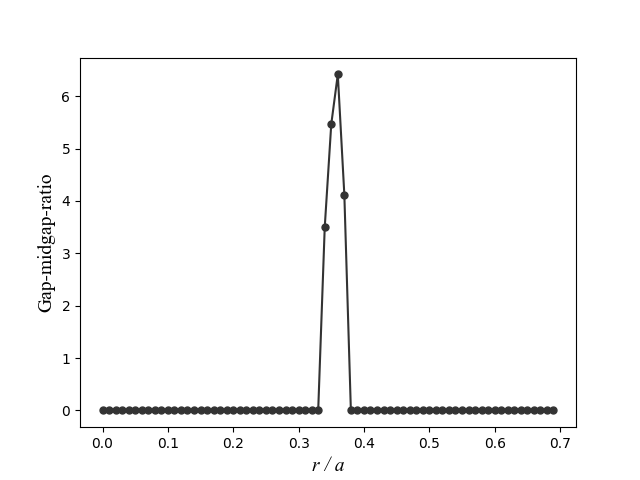
\includegraphics[width=0.8\linewidth]{results/inv_opals.png}
  \caption{逆オパール構造の球の半径を変化させた際のギャップ-ミッドギャップ比の変化}
  \label{fig:inv_opal}
\end{figure}

$0.34 \leq r / a \leq 0.37$の範囲でのみバンドギャップが確認でき、その中で最大値をとる$r / a = 0.36$のときのギャップ-ミッドギャップ比は最大となりその値は$6.41675 \% $であった。



\subsection{ウッドパイル構造}
ウッドパイル構造中の棒状誘電体の幅を徐々に変化させていった際のギャップ-ミッドギャップ比の変化を図\ref{fig:woodpile}に示す。

\begin{figure}[htbp]
  \centering
  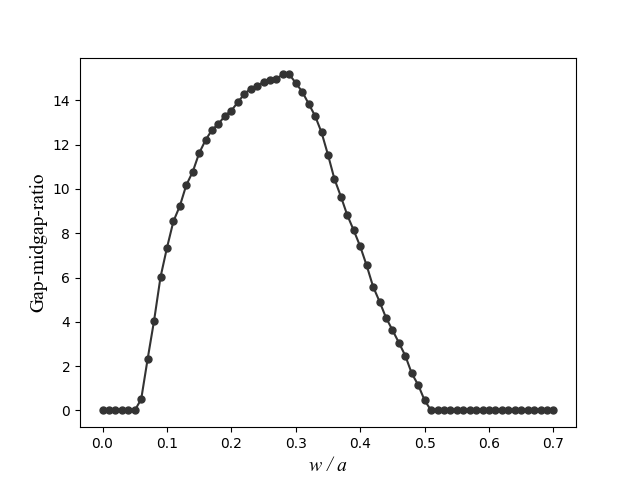
\includegraphics[width=0.8\linewidth]{results/woodpile.png}
  \caption{ウッドパイル構造の棒状誘電体の幅を変化させた際のギャップ-ミッドギャップ比の変化}
  \label{fig:woodpile}
\end{figure}

誘電体棒幅$w = 0.28$で最大となり、ギャップ-ミッドギャップ比は$15.17613425 \%$となった。

\subsection{ヤブロノバイト構造}
ヤブロノバイト構造中の空気柱の半径を連続的に変化させた際のギャップ-ミッドギャップ比の変化を図\ref{fig:yablonovite}に示す。
\begin{figure}[htbp]
  \centering
  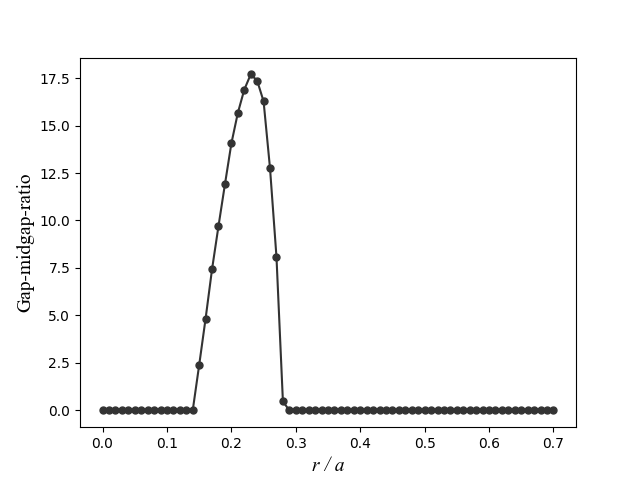
\includegraphics[width=0.8\linewidth]{results/yablonovite.png}
  \caption{ヤブロノバイト構造の空気柱の半径を変化させた際のギャップ-ミッドギャップ比の変化}
  \label{fig:yablonovite}
\end{figure}

\subsection{2次元構造の積み重ね}
2次元結晶の積み重ねによって3次元結晶を作成した際のギャップ-ミッドギャップ比の変化を図\ref{fig:stack-crystals}に示す。
\begin{figure}[htbp]
  \centering
  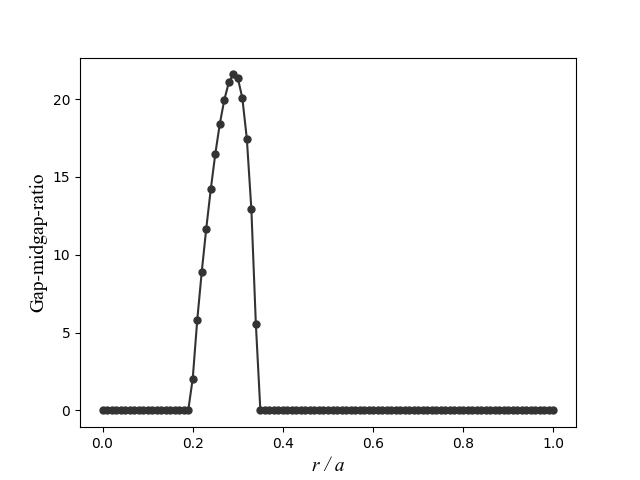
\includegraphics[width=0.8\linewidth]{results/stack-crystals.png}
  \caption{2次元結晶の積み重ねによって作成した3次元結晶のギャップ-ミッドギャップ比の変化}
  \label{fig:stack-crystals}
\end{figure}


\section{考察}
\subsection{逆オパール構造}
\subsection{ウッドパイル構造}
\subsection{ヤブロノバイト構造}
\subsection{2次元構造の積み重ね}

\end{document}